\section{Uniformly Controlled Rotations}
\label{sec:multiplexed-rotations}

Implementing a series of uniformly controlled rotations is a common subroutine used in this work.
In this section, we discuss the cost and explicit circuit compilation for a series of uniformly controlled rotations around the same axis (but different angles) are applied on the same qubit:
\begin{equation}
    \sum_{l=0}^{L - 1} \ket{l} \ket{\phi} \rightarrow \sum_{l=0}^{L - 1} \ket{l} R_a (\alpha_l) \ket{\phi}
\end{equation}

Möttönen et. al \cite{mottonen2004transformation}, provide a construction for \textit{uncontrolled} uniformly controlled rotations.
This construction is only defined when the number of rotations ($L$) is explicitly a power of $2$, however, if fewer rotations are required, then this can be achieved by padding with zero-angle rotations.

In this construction, the rotation angles are classically preprocessed based on the Gray code (Eq. 3 of \cite{mottonen2004transformation}):
\begin{equation}
    \begin{bmatrix}
        \theta_{0} \\
        \theta_{1} \\
        \vdots \\
        \theta_{L - 1}
    \end{bmatrix} = M \begin{bmatrix}
        \alpha_{0} \\
        \alpha_{1} \\
        \vdots \\
        \alpha_{L - 1}
    \end{bmatrix}
\end{equation}
where $M$ is a matrix transformation defined by:
\begin{equation}
    M_{i, j} = L^{-1} (-1)^{b_{j} . g_{i}}
\end{equation}
where $b_j$ is the binary representation of the integer $j$, $g_i$ is the Gray code representation of the integer $i$, and $b_{j} . g_{i}$ is the bitwise inner product of $b_{j}$ and $g_{i}$.

\begin{figure*}
    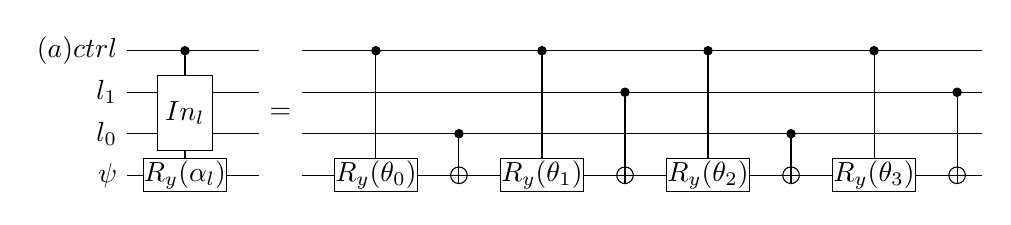
\begin{tikzpicture}[scale=1.000000,x=1pt,y=1pt]
\filldraw[color=white] (0.000000, -7.500000) rectangle (309.000000, 52.500000);
% Drawing wires
% Line 1: ctrl W \text{(a) }ctrl
\draw[color=black] (0.000000,45.000000) -- (309.000000,45.000000);
\draw[color=black] (0.000000,45.000000) node[left] {$\text{(a) }ctrl$};
% Line 2: l1 W l_1
\draw[color=black] (0.000000,30.000000) -- (309.000000,30.000000);
\draw[color=black] (0.000000,30.000000) node[left] {$l_1$};
% Line 3: l0 W l_0
\draw[color=black] (0.000000,15.000000) -- (309.000000,15.000000);
\draw[color=black] (0.000000,15.000000) node[left] {$l_0$};
% Line 4: sys W \psi
\draw[color=black] (0.000000,0.000000) -- (309.000000,0.000000);
\draw[color=black] (0.000000,0.000000) node[left] {$\psi$};
% Done with wires; drawing gates
% Line 6: l1 l0 G:width=20 $In_l$ sys G:width=30 $R_y (\alpha_l)$ ctrl
\draw (21.000000,45.000000) -- (21.000000,0.000000);
\begin{scope}
\draw[fill=white] (21.000000, 22.500000) +(-45.000000:14.142136pt and 19.091883pt) -- +(45.000000:14.142136pt and 19.091883pt) -- +(135.000000:14.142136pt and 19.091883pt) -- +(225.000000:14.142136pt and 19.091883pt) -- cycle;
\clip (21.000000, 22.500000) +(-45.000000:14.142136pt and 19.091883pt) -- +(45.000000:14.142136pt and 19.091883pt) -- +(135.000000:14.142136pt and 19.091883pt) -- +(225.000000:14.142136pt and 19.091883pt) -- cycle;
\draw (21.000000, 22.500000) node {$In_l$};
\end{scope}
\begin{scope}
\draw[fill=white] (21.000000, -0.000000) +(-45.000000:21.213203pt and 8.485281pt) -- +(45.000000:21.213203pt and 8.485281pt) -- +(135.000000:21.213203pt and 8.485281pt) -- +(225.000000:21.213203pt and 8.485281pt) -- cycle;
\clip (21.000000, -0.000000) +(-45.000000:21.213203pt and 8.485281pt) -- +(45.000000:21.213203pt and 8.485281pt) -- +(135.000000:21.213203pt and 8.485281pt) -- +(225.000000:21.213203pt and 8.485281pt) -- cycle;
\draw (21.000000, -0.000000) node {$R_y (\alpha_l)$};
\end{scope}
\filldraw (21.000000, 45.000000) circle(1.500000pt);
% Line 8: =
\draw[fill=white,color=white] (48.000000, -6.000000) rectangle (63.000000, 51.000000);
\draw (55.500000, 22.500000) node {$=$};
% Line 10: sys G width=30 $R_y (\theta_0)$ ctrl
\draw (90.000000,45.000000) -- (90.000000,0.000000);
\begin{scope}
\draw[fill=white] (90.000000, -0.000000) +(-45.000000:21.213203pt and 8.485281pt) -- +(45.000000:21.213203pt and 8.485281pt) -- +(135.000000:21.213203pt and 8.485281pt) -- +(225.000000:21.213203pt and 8.485281pt) -- cycle;
\clip (90.000000, -0.000000) +(-45.000000:21.213203pt and 8.485281pt) -- +(45.000000:21.213203pt and 8.485281pt) -- +(135.000000:21.213203pt and 8.485281pt) -- +(225.000000:21.213203pt and 8.485281pt) -- cycle;
\draw (90.000000, -0.000000) node {$R_y (\theta_0)$};
\end{scope}
\filldraw (90.000000, 45.000000) circle(1.500000pt);
% Line 11: +sys l0
\draw (120.000000,15.000000) -- (120.000000,0.000000);
\begin{scope}
\draw[fill=white] (120.000000, 0.000000) circle(3.000000pt);
\clip (120.000000, 0.000000) circle(3.000000pt);
\draw (117.000000, 0.000000) -- (123.000000, 0.000000);
\draw (120.000000, -3.000000) -- (120.000000, 3.000000);
\end{scope}
\filldraw (120.000000, 15.000000) circle(1.500000pt);
% Line 12: sys G width=30 $R_y (\theta_1)$ ctrl
\draw (150.000000,45.000000) -- (150.000000,0.000000);
\begin{scope}
\draw[fill=white] (150.000000, -0.000000) +(-45.000000:21.213203pt and 8.485281pt) -- +(45.000000:21.213203pt and 8.485281pt) -- +(135.000000:21.213203pt and 8.485281pt) -- +(225.000000:21.213203pt and 8.485281pt) -- cycle;
\clip (150.000000, -0.000000) +(-45.000000:21.213203pt and 8.485281pt) -- +(45.000000:21.213203pt and 8.485281pt) -- +(135.000000:21.213203pt and 8.485281pt) -- +(225.000000:21.213203pt and 8.485281pt) -- cycle;
\draw (150.000000, -0.000000) node {$R_y (\theta_1)$};
\end{scope}
\filldraw (150.000000, 45.000000) circle(1.500000pt);
% Line 13: +sys l1
\draw (180.000000,30.000000) -- (180.000000,0.000000);
\begin{scope}
\draw[fill=white] (180.000000, 0.000000) circle(3.000000pt);
\clip (180.000000, 0.000000) circle(3.000000pt);
\draw (177.000000, 0.000000) -- (183.000000, 0.000000);
\draw (180.000000, -3.000000) -- (180.000000, 3.000000);
\end{scope}
\filldraw (180.000000, 30.000000) circle(1.500000pt);
% Line 14: sys G width=30 $R_y (\theta_2)$ ctrl
\draw (210.000000,45.000000) -- (210.000000,0.000000);
\begin{scope}
\draw[fill=white] (210.000000, -0.000000) +(-45.000000:21.213203pt and 8.485281pt) -- +(45.000000:21.213203pt and 8.485281pt) -- +(135.000000:21.213203pt and 8.485281pt) -- +(225.000000:21.213203pt and 8.485281pt) -- cycle;
\clip (210.000000, -0.000000) +(-45.000000:21.213203pt and 8.485281pt) -- +(45.000000:21.213203pt and 8.485281pt) -- +(135.000000:21.213203pt and 8.485281pt) -- +(225.000000:21.213203pt and 8.485281pt) -- cycle;
\draw (210.000000, -0.000000) node {$R_y (\theta_2)$};
\end{scope}
\filldraw (210.000000, 45.000000) circle(1.500000pt);
% Line 15: +sys l0
\draw (240.000000,15.000000) -- (240.000000,0.000000);
\begin{scope}
\draw[fill=white] (240.000000, 0.000000) circle(3.000000pt);
\clip (240.000000, 0.000000) circle(3.000000pt);
\draw (237.000000, 0.000000) -- (243.000000, 0.000000);
\draw (240.000000, -3.000000) -- (240.000000, 3.000000);
\end{scope}
\filldraw (240.000000, 15.000000) circle(1.500000pt);
% Line 16: sys G width=30 $R_y (\theta_3)$ ctrl
\draw (270.000000,45.000000) -- (270.000000,0.000000);
\begin{scope}
\draw[fill=white] (270.000000, -0.000000) +(-45.000000:21.213203pt and 8.485281pt) -- +(45.000000:21.213203pt and 8.485281pt) -- +(135.000000:21.213203pt and 8.485281pt) -- +(225.000000:21.213203pt and 8.485281pt) -- cycle;
\clip (270.000000, -0.000000) +(-45.000000:21.213203pt and 8.485281pt) -- +(45.000000:21.213203pt and 8.485281pt) -- +(135.000000:21.213203pt and 8.485281pt) -- +(225.000000:21.213203pt and 8.485281pt) -- cycle;
\draw (270.000000, -0.000000) node {$R_y (\theta_3)$};
\end{scope}
\filldraw (270.000000, 45.000000) circle(1.500000pt);
% Line 17: +sys l1
\draw (300.000000,30.000000) -- (300.000000,0.000000);
\begin{scope}
\draw[fill=white] (300.000000, 0.000000) circle(3.000000pt);
\clip (300.000000, 0.000000) circle(3.000000pt);
\draw (297.000000, 0.000000) -- (303.000000, 0.000000);
\draw (300.000000, -3.000000) -- (300.000000, 3.000000);
\end{scope}
\filldraw (300.000000, 30.000000) circle(1.500000pt);
% Done with gates; drawing ending labels
% Done with ending labels; drawing cut lines and comments
% Done with comments
\end{tikzpicture}

    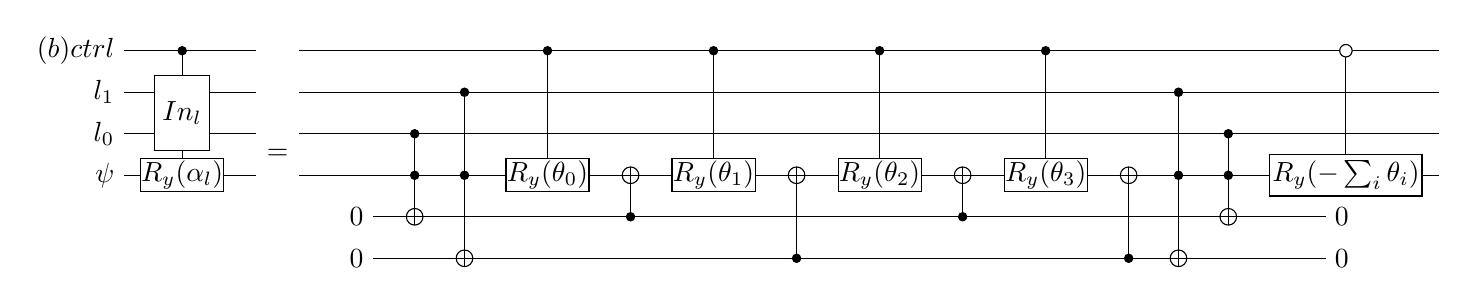
\begin{tikzpicture}[scale=1.000000,x=1pt,y=1pt]
\filldraw[color=white] (0.000000, -7.500000) rectangle (475.000000, 82.500000);
% Drawing wires
% Line 1: ctrl W \text{(b) }ctrl
\draw[color=black] (0.000000,75.000000) -- (475.000000,75.000000);
\draw[color=black] (0.000000,75.000000) node[left] {$\text{(b) }ctrl$};
% Line 2: l1 W l_1
\draw[color=black] (0.000000,60.000000) -- (475.000000,60.000000);
\draw[color=black] (0.000000,60.000000) node[left] {$l_1$};
% Line 3: l0 W l_0
\draw[color=black] (0.000000,45.000000) -- (475.000000,45.000000);
\draw[color=black] (0.000000,45.000000) node[left] {$l_0$};
% Line 4: sys W \psi
\draw[color=black] (0.000000,30.000000) -- (475.000000,30.000000);
\draw[color=black] (0.000000,30.000000) node[left] {$\psi$};
% Line 5: c0 W 0 0
\draw[color=black] (82.500000,15.000000) -- (441.500000,15.000000);
% Line 6: c1 W 0 0
\draw[color=black] (82.500000,0.000000) -- (441.500000,0.000000);
% Done with wires; drawing gates
% Line 8: sys G:width=30 $R_y (\alpha_l)$ l1 l0 G:width=20 $In_l$ ctrl
\draw (21.000000,75.000000) -- (21.000000,30.000000);
\begin{scope}
\draw[fill=white] (21.000000, 30.000000) +(-45.000000:21.213203pt and 8.485281pt) -- +(45.000000:21.213203pt and 8.485281pt) -- +(135.000000:21.213203pt and 8.485281pt) -- +(225.000000:21.213203pt and 8.485281pt) -- cycle;
\clip (21.000000, 30.000000) +(-45.000000:21.213203pt and 8.485281pt) -- +(45.000000:21.213203pt and 8.485281pt) -- +(135.000000:21.213203pt and 8.485281pt) -- +(225.000000:21.213203pt and 8.485281pt) -- cycle;
\draw (21.000000, 30.000000) node {$R_y (\alpha_l)$};
\end{scope}
\begin{scope}
\draw[fill=white] (21.000000, 52.500000) +(-45.000000:14.142136pt and 19.091883pt) -- +(45.000000:14.142136pt and 19.091883pt) -- +(135.000000:14.142136pt and 19.091883pt) -- +(225.000000:14.142136pt and 19.091883pt) -- cycle;
\clip (21.000000, 52.500000) +(-45.000000:14.142136pt and 19.091883pt) -- +(45.000000:14.142136pt and 19.091883pt) -- +(135.000000:14.142136pt and 19.091883pt) -- +(225.000000:14.142136pt and 19.091883pt) -- cycle;
\draw (21.000000, 52.500000) node {$In_l$};
\end{scope}
\filldraw (21.000000, 75.000000) circle(1.500000pt);
% Line 10: =
\draw[fill=white,color=white] (48.000000, -6.000000) rectangle (63.000000, 81.000000);
\draw (55.500000, 37.500000) node {$=$};
% Line 12: c0 c1 START
\draw[color=black] (90.000000,15.000000) node[fill=white,left,minimum height=15.000000pt,minimum width=15.000000pt,inner sep=0pt] {\phantom{$0$}};
\draw[color=black] (90.000000,15.000000) node[left] {$0$};
\draw[color=black] (90.000000,0.000000) node[fill=white,left,minimum height=15.000000pt,minimum width=15.000000pt,inner sep=0pt] {\phantom{$0$}};
\draw[color=black] (90.000000,0.000000) node[left] {$0$};
% Line 13: +c0 sys l0
\draw (105.000000,45.000000) -- (105.000000,15.000000);
\begin{scope}
\draw[fill=white] (105.000000, 15.000000) circle(3.000000pt);
\clip (105.000000, 15.000000) circle(3.000000pt);
\draw (102.000000, 15.000000) -- (108.000000, 15.000000);
\draw (105.000000, 12.000000) -- (105.000000, 18.000000);
\end{scope}
\filldraw (105.000000, 30.000000) circle(1.500000pt);
\filldraw (105.000000, 45.000000) circle(1.500000pt);
% Line 14: +c1 sys l1
\draw (123.000000,60.000000) -- (123.000000,0.000000);
\begin{scope}
\draw[fill=white] (123.000000, 0.000000) circle(3.000000pt);
\clip (123.000000, 0.000000) circle(3.000000pt);
\draw (120.000000, 0.000000) -- (126.000000, 0.000000);
\draw (123.000000, -3.000000) -- (123.000000, 3.000000);
\end{scope}
\filldraw (123.000000, 30.000000) circle(1.500000pt);
\filldraw (123.000000, 60.000000) circle(1.500000pt);
% Line 16: sys G width=30 $R_y (\theta_0)$ ctrl
\draw (153.000000,75.000000) -- (153.000000,30.000000);
\begin{scope}
\draw[fill=white] (153.000000, 30.000000) +(-45.000000:21.213203pt and 8.485281pt) -- +(45.000000:21.213203pt and 8.485281pt) -- +(135.000000:21.213203pt and 8.485281pt) -- +(225.000000:21.213203pt and 8.485281pt) -- cycle;
\clip (153.000000, 30.000000) +(-45.000000:21.213203pt and 8.485281pt) -- +(45.000000:21.213203pt and 8.485281pt) -- +(135.000000:21.213203pt and 8.485281pt) -- +(225.000000:21.213203pt and 8.485281pt) -- cycle;
\draw (153.000000, 30.000000) node {$R_y (\theta_0)$};
\end{scope}
\filldraw (153.000000, 75.000000) circle(1.500000pt);
% Line 17: +sys c0
\draw (183.000000,30.000000) -- (183.000000,15.000000);
\begin{scope}
\draw[fill=white] (183.000000, 30.000000) circle(3.000000pt);
\clip (183.000000, 30.000000) circle(3.000000pt);
\draw (180.000000, 30.000000) -- (186.000000, 30.000000);
\draw (183.000000, 27.000000) -- (183.000000, 33.000000);
\end{scope}
\filldraw (183.000000, 15.000000) circle(1.500000pt);
% Line 18: sys G width=30 $R_y (\theta_1)$ ctrl
\draw (213.000000,75.000000) -- (213.000000,30.000000);
\begin{scope}
\draw[fill=white] (213.000000, 30.000000) +(-45.000000:21.213203pt and 8.485281pt) -- +(45.000000:21.213203pt and 8.485281pt) -- +(135.000000:21.213203pt and 8.485281pt) -- +(225.000000:21.213203pt and 8.485281pt) -- cycle;
\clip (213.000000, 30.000000) +(-45.000000:21.213203pt and 8.485281pt) -- +(45.000000:21.213203pt and 8.485281pt) -- +(135.000000:21.213203pt and 8.485281pt) -- +(225.000000:21.213203pt and 8.485281pt) -- cycle;
\draw (213.000000, 30.000000) node {$R_y (\theta_1)$};
\end{scope}
\filldraw (213.000000, 75.000000) circle(1.500000pt);
% Line 19: +sys c1
\draw (243.000000,30.000000) -- (243.000000,0.000000);
\begin{scope}
\draw[fill=white] (243.000000, 30.000000) circle(3.000000pt);
\clip (243.000000, 30.000000) circle(3.000000pt);
\draw (240.000000, 30.000000) -- (246.000000, 30.000000);
\draw (243.000000, 27.000000) -- (243.000000, 33.000000);
\end{scope}
\filldraw (243.000000, 0.000000) circle(1.500000pt);
% Line 20: sys G width=30 $R_y (\theta_2)$ ctrl
\draw (273.000000,75.000000) -- (273.000000,30.000000);
\begin{scope}
\draw[fill=white] (273.000000, 30.000000) +(-45.000000:21.213203pt and 8.485281pt) -- +(45.000000:21.213203pt and 8.485281pt) -- +(135.000000:21.213203pt and 8.485281pt) -- +(225.000000:21.213203pt and 8.485281pt) -- cycle;
\clip (273.000000, 30.000000) +(-45.000000:21.213203pt and 8.485281pt) -- +(45.000000:21.213203pt and 8.485281pt) -- +(135.000000:21.213203pt and 8.485281pt) -- +(225.000000:21.213203pt and 8.485281pt) -- cycle;
\draw (273.000000, 30.000000) node {$R_y (\theta_2)$};
\end{scope}
\filldraw (273.000000, 75.000000) circle(1.500000pt);
% Line 21: +sys c0
\draw (303.000000,30.000000) -- (303.000000,15.000000);
\begin{scope}
\draw[fill=white] (303.000000, 30.000000) circle(3.000000pt);
\clip (303.000000, 30.000000) circle(3.000000pt);
\draw (300.000000, 30.000000) -- (306.000000, 30.000000);
\draw (303.000000, 27.000000) -- (303.000000, 33.000000);
\end{scope}
\filldraw (303.000000, 15.000000) circle(1.500000pt);
% Line 22: sys G width=30 $R_y (\theta_3)$ ctrl
\draw (333.000000,75.000000) -- (333.000000,30.000000);
\begin{scope}
\draw[fill=white] (333.000000, 30.000000) +(-45.000000:21.213203pt and 8.485281pt) -- +(45.000000:21.213203pt and 8.485281pt) -- +(135.000000:21.213203pt and 8.485281pt) -- +(225.000000:21.213203pt and 8.485281pt) -- cycle;
\clip (333.000000, 30.000000) +(-45.000000:21.213203pt and 8.485281pt) -- +(45.000000:21.213203pt and 8.485281pt) -- +(135.000000:21.213203pt and 8.485281pt) -- +(225.000000:21.213203pt and 8.485281pt) -- cycle;
\draw (333.000000, 30.000000) node {$R_y (\theta_3)$};
\end{scope}
\filldraw (333.000000, 75.000000) circle(1.500000pt);
% Line 23: +sys c1
\draw (363.000000,30.000000) -- (363.000000,0.000000);
\begin{scope}
\draw[fill=white] (363.000000, 30.000000) circle(3.000000pt);
\clip (363.000000, 30.000000) circle(3.000000pt);
\draw (360.000000, 30.000000) -- (366.000000, 30.000000);
\draw (363.000000, 27.000000) -- (363.000000, 33.000000);
\end{scope}
\filldraw (363.000000, 0.000000) circle(1.500000pt);
% Line 25: +c1 sys l1
\draw (381.000000,60.000000) -- (381.000000,0.000000);
\begin{scope}
\draw[fill=white] (381.000000, 0.000000) circle(3.000000pt);
\clip (381.000000, 0.000000) circle(3.000000pt);
\draw (378.000000, 0.000000) -- (384.000000, 0.000000);
\draw (381.000000, -3.000000) -- (381.000000, 3.000000);
\end{scope}
\filldraw (381.000000, 30.000000) circle(1.500000pt);
\filldraw (381.000000, 60.000000) circle(1.500000pt);
% Line 26: +c0 sys l0
\draw (399.000000,45.000000) -- (399.000000,15.000000);
\begin{scope}
\draw[fill=white] (399.000000, 15.000000) circle(3.000000pt);
\clip (399.000000, 15.000000) circle(3.000000pt);
\draw (396.000000, 15.000000) -- (402.000000, 15.000000);
\draw (399.000000, 12.000000) -- (399.000000, 18.000000);
\end{scope}
\filldraw (399.000000, 30.000000) circle(1.500000pt);
\filldraw (399.000000, 45.000000) circle(1.500000pt);
% Line 27: c0 c1 END
\draw[color=black] (434.000000,15.000000) node[fill=white,right,minimum height=15.000000pt,minimum width=15.000000pt,inner sep=0pt] {\phantom{$0$}};
\draw[color=black] (434.000000,15.000000) node[right] {$0$};
\draw[color=black] (434.000000,0.000000) node[fill=white,right,minimum height=15.000000pt,minimum width=15.000000pt,inner sep=0pt] {\phantom{$0$}};
\draw[color=black] (434.000000,0.000000) node[right] {$0$};
% Line 29: sys G:width=55:height=15 $R_y(-\sum_i \theta_i)$ -ctrl
\draw (441.500000,75.000000) -- (441.500000,30.000000);
\begin{scope}
\draw[fill=white] (441.500000, 30.000000) +(-45.000000:38.890873pt and 10.606602pt) -- +(45.000000:38.890873pt and 10.606602pt) -- +(135.000000:38.890873pt and 10.606602pt) -- +(225.000000:38.890873pt and 10.606602pt) -- cycle;
\clip (441.500000, 30.000000) +(-45.000000:38.890873pt and 10.606602pt) -- +(45.000000:38.890873pt and 10.606602pt) -- +(135.000000:38.890873pt and 10.606602pt) -- +(225.000000:38.890873pt and 10.606602pt) -- cycle;
\draw (441.500000, 30.000000) node {$R_y(-\sum_i \theta_i)$};
\end{scope}
\draw[fill=white] (441.500000, 75.000000) circle(2.250000pt);
% Done with gates; drawing ending labels
% Done with ending labels; drawing cut lines and comments
% Done with comments
\end{tikzpicture}

    \caption{
        \textbf{Controlled Uniformly Controlled Rotations}
        Two implementations for controlling a series of uniformly controlled rotations are shown.
        In (a), a naive implementation is shown which doubles the number of arbitrary rotations required.
        The implementation shown in (b) uses only one additional controlled rotation and $\log_2 L$ Toffoli gates, but requires $\log_2 L$ clean ancillae.
    }
    \label{fig:controlled-multiplexed-rotations}
\end{figure*}

However, in this work we require the use of a \textit{controlled} series of uniformly controlled rotations.
Naively, this can be implemented by controlling each of the arbitrary rotations in the construction given by Möttönen et al. \cite{mottonen2004transformation}.
An example circuit diagram for this construction is shown in subfigure \ref{fig:controlled-multiplexed-rotations}a.
Since each controlled rotation can be implemented by two uncontrolled rotations, this compilation strategy uses $2L$ uncontrolled arbitrary rotations.

An alternative approach which uses $4 \log_2 L$ T gates, $L + 3$ arbitrary rotations, and $\log_2 L$ clean ancillae is shown in subfigure \ref{fig:controlled-multiplexed-rotations}b.
In this construction, the temporary logical-AND of each qubit in the index register and the control qubit is computed using $\log_2 L$ Toffoli gates.
CNOTs from these clean ancillae then conjugate each of the arbitrary rotations which are left uncontrolled.
When the control is on, this fully recovers the construction given by Möttönen et. al.

However, when the control is off, the uncontrolled arbitrary rotations are still applied, resulting an undesired rotation of angle $\sum_{i} (\theta_i)$.
This undesired rotation can then be undone using one $0$-controlled rotation of angle $- \sum_{i} (\theta_i)$.
